\documentclass[11pt,a4paper]{article}
\usepackage[margin=22mm]{geometry}
\usepackage[T1]{fontenc}
\usepackage{lmodern,amsmath,amssymb,booktabs,longtable,array,graphicx,tikz,xcolor,hyperref}
\usetikzlibrary{arrows.meta,positioning,calc,shapes.geometric}
\hypersetup{pdftitle={VLSI Testing - 2020 Final - Reconstructed Questions and Solutions},pdfauthor={},colorlinks=true,linkcolor=blue,urlcolor=blue}
\newcommand{\question}[1]{\paragraph{Question.}#1}
\newcommand{\answer}{\paragraph{Solution.}}
\newcommand{\bits}[1]{\texttt{#1}}
\newcommand{\march}[1]{\ensuremath{\left\{#1\right\}}}
\newcommand{\up}{\mathord{\uparrow}}
\newcommand{\dn}{\mathord{\downarrow}}
\newcommand{\any}{\mathord{\updownarrow}}
\setlength{\emergencystretch}{2em}
\title{VLSI Testing\\2020 Final\\Reconstructed Questions and Solutions}
\author{}
\date{}
\begin{document}
\maketitle
\noindent This study edition rebuilds the three supplied exam pages as editable text, tables, and diagrams. Questions are paraphrased without changing their technical conditions or printed point values. Solutions are independently reasoned and checked where a finite model is practical. The accompanying student material serves only as a reference. In particular, the BILBO mode interpretation and the TAM routing constraints are examined rather than copied from the handwritten answers.
\par\medskip
\noindent\textbf{Notation.} In a March element, $wD$ writes data background $D$ and $rD$ reads and compares against $D$. Arrows denote increasing, decreasing, or either address order. $N$ is the number of addressed words. Complements and XOR operations in Boolean recurrences act bitwise. Fault-coverage statements refer to the conventional single-fault models named in the question.
\section{Short questions (30 points)}
\subsection{Must-repair allocation (5 points)}
\question{Heuristic redundancy analysis commonly has a must-repair phase followed by a final-repair phase. State the allocation rules of the must-repair phase.}
\answer Let $R$ and $C$ be the remaining spare-row and spare-column counts. If one faulty row contains faults in more than $C$ distinct columns, column replacement alone cannot cover them. That row must receive a spare row. Similarly, a column containing faults in more than $R$ distinct rows must receive a spare column. After an allocation, remove the faults it covers, decrease the relevant spare count, and repeat the rules with the updated counts. A required allocation with no corresponding spare available proves failure under the available resources. When neither rule applies, the final-repair phase chooses how to cover the remaining faults. A heuristic choice in that later phase need not find every feasible allocation.

\subsection{Solid backgrounds in word memories (5 points)}
\question{Why does a bit-oriented March test using only all-zero and all-one backgrounds fail to cover all coupling faults in a word-oriented memory?}
\answer A word write changes several cells together. Solid backgrounds give the same value to every bit in a word, so they do not distinguish a victim bit from an aggressor bit at another position. Intra-word coupling that requires opposite states, or a transition of one bit while another has a particular state, can escape those backgrounds or be masked by simultaneous writes. Complementary striped backgrounds separate pairs of bit positions. Inter-word coupling and intra-word coupling must both be considered when converting the bit-oriented test.

\subsection{Built-in self-diagnosis output (5 points)}
\question{What information should a built-in self-diagnosis circuit export for subsequent diagnosis analysis?}
\answer Export the failing address, the failing bit positions or the expected-data XOR actual-data mask, and enough test context to interpret a failure. Useful context includes the applied background, the read/write operation, the March element or cycle, and the observed/expected values. This permits reconstruction of faulty rows and columns and distinguishes different manifestations of a fault. If information is compressed or stored in a bounded buffer, export its validity and overflow status. The diagnosis circuit measures the failures. The redundancy analyzer separately decides which spare rows or columns to allocate.

\subsection{Concurrent and non-concurrent online BIST (5 points)}
\question{Explain concurrent and non-concurrent online BIST.}
\answer Concurrent online BIST checks a circuit while its normal functional operations continue, for example by monitoring functional responses. Non-concurrent online BIST schedules dedicated test activity in idle intervals or temporarily suspends the relevant normal operation. Both belong to online testing, but the second needs a testing interval that does not overlap the protected function's normal work.

\subsection{DRAM retention test (5 points)}
\question{A DRAM has a 32 ms refresh period. Give a March test that detects both stuck-at polarities and the modeled data-retention faults.}
\answer Disable refresh for the tested cells during each retention interval. Let $t_h$ be at least 32 ms, with an appropriate implementation margin. One test is
\[
\march{\any(w0);\ \mathrm{wait}(t_h);\ \up(r0,w1);\ \mathrm{wait}(t_h);\ \up(r1)}.
\]
The first write and subsequent zero comparison detect cells that cannot store zero, including stuck-at-one faults. The one write and final one comparison detect stuck-at-zero faults. Each polarity is also held without refresh before it is read. Wait until after the entire preceding write pass has finished, so even the last-written cell receives the required hold time. The access cost is $4N$, plus two retention waits. This establishes coverage of the specified retention model at the chosen hold condition, not every possible analog leakage behavior or operating condition.

\subsection{Fuse and antifuse (5 points)}
\question{How do fuse and antifuse one-time programmable memories differ?}
\answer A fuse starts as a conducting link and programming opens that link. An antifuse starts as an insulating connection and programming creates a conducting path. Both preserve the programmed state without power and are normally one-time programmable. The sense circuitry interprets the opposite initial and programmed electrical states accordingly.

\section{Eight-bit word-oriented March C-minus (10 points)}
\question{Convert the supplied March C-minus test into a test for eight-bit words that covers inversion, idempotent, and state coupling faults.}
\answer A straightforward conversion uses four standard backgrounds and their complements:
\[
D\in\{\bits{00000000},\bits{01010101},\bits{00110011},\bits{00001111}\}.
\]
For each $D$, execute the complete sequence
\[
C^-(D)=\left\{\begin{aligned}
&\any(wD);\ \up(rD,w\overline D);\ \up(r\overline D,wD);\\
&\dn(rD,w\overline D);\ \dn(r\overline D,wD);\ \any(rD)
\end{aligned}\right\}.
\]
This gives $4\times10N=40N$ word operations. It is a straightforward construction rather than an optimized compact conversion.

The solid background supplies equal-state combinations. For any two distinct bit positions, their three-bit position indices differ in at least one coordinate. One of the striped backgrounds therefore puts those two positions at opposite values, and its complement reverses their values. The complete set supplies the required equal and opposite pair conditions. Running both upward and downward March elements supplies both address orders for inter-word aggressor/victim relationships. Together these are the conventional background and ordering conditions for the named unlinked coupling-fault classes.

\begin{center}
\begin{tabular}{cll}
\toprule Background & Complement & Separation of bit positions\\\midrule
00000000&11111111&Equal-state reference\\
01010101&10101010&Alternating adjacent positions\\
00110011&11001100&Groups of two positions\\
00001111&11110000&Groups of four positions\\
\bottomrule
\end{tabular}
\end{center}

\section{Components of RAM BISR (10 points)}
\question{Explain the built-in self-test, built-in redundancy analyzer, and reconfiguration mechanism in a RAM self-repair system.}
\answer The BIST controller applies memory operations, generates addresses and data, compares the read data, and records a fault map or repair-relevant failure information. The built-in redundancy analyzer (BIRA) uses that information and the available spare resources to produce a row/column allocation, or to report that the selected repair strategy has failed. The reconfiguration mechanism stores and applies the allocation, redirecting accesses from faulty locations to spare rows, columns, or words. Repeating the test after reconfiguration checks the resulting memory operation.
\begin{figure}[ht]\centering
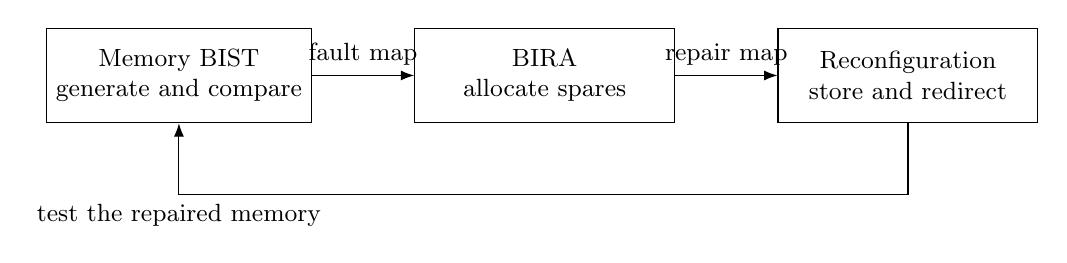
\begin{tikzpicture}[>=Latex,b/.style={draw,align=center,minimum width=33mm,minimum height=12mm},font=\small]
\node[b] (bist) {Memory BIST\\generate and compare};
\node[b,right=13mm of bist] (bira) {BIRA\\allocate spares};
\node[b,right=13mm of bira] (config) {Reconfiguration\\store and redirect};
\draw[->](bist)--node[above]{fault map}(bira);
\draw[->](bira)--node[above]{repair map}(config);
\draw[->](config.south)--++(0,-9mm)-|node[pos=.5,below]{test the repaired memory}(bist.south);
\end{tikzpicture}
\caption{Functions in a memory self-repair flow.}
\end{figure}

\section{Repair configuration and fuse sensing (15 points)}
\subsection{Three reconfiguration mechanisms (10 points)}
\question{List three memory-repair reconfiguration mechanisms and give their advantages and disadvantages.}
\answer The course distinction is soft, firm, and hard reconfiguration.
\begin{center}\small
\begin{tabular}{>{\raggedright\arraybackslash}p{18mm}>{\raggedright\arraybackslash}p{40mm}>{\raggedright\arraybackslash}p{40mm}>{\raggedright\arraybackslash}p{42mm}}
\toprule Type&Repair information&Advantages&Limitations\\\midrule
Soft&Volatile flip-flops or configuration registers&Can recompute and reload repair maps more than once; little nonvolatile-storage overhead&Map is lost at power-off, so boot may require retest and analysis. A latent defect arising between repair runs remains until another run.\\[1mm]
Firm&Programmable nonvolatile memory&Retains a repair map and can support repeated repair updates when the storage technology is rewritable&Needs the nonvolatile storage and its programming support, often including programming voltages and circuitry.\\[1mm]
Hard&Permanently programmed fuses or equivalent links&Retains the map and permits short setup by loading or sensing it&One-time repair configuration cannot generally be revised after the relevant links are consumed.\\
\bottomrule
\end{tabular}\end{center}
The exact area and setup-time tradeoffs depend on the chosen implementation. These mechanisms concern how the repair map is retained and activated, rather than the particular address comparator or data multiplexer topology.

\subsection{Read the fuse into a flip-flop (5 points)}
\question{Explain how the shown fuse cell transfers its stored state to the D flip-flop. The fuse connects node $a$ to a pull-down NMOS. Read controls the upper PMOS and lower NMOS, Reset discharges $a$, and a Read-controlled multiplexer selects either feedback $Q$ or node $a$.}
\begin{figure}[ht]\centering
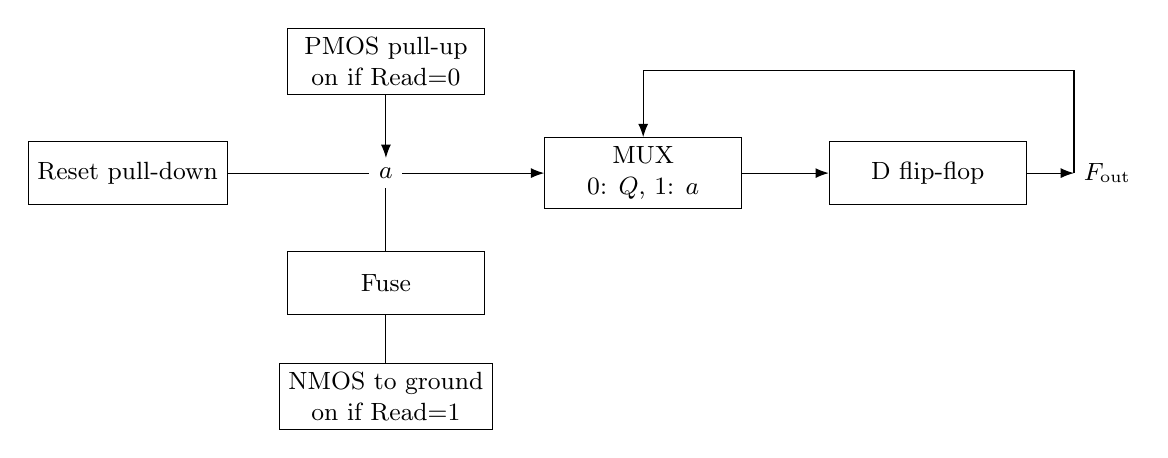
\begin{tikzpicture}[>=Latex,font=\small,b/.style={draw,align=center,minimum height=8mm,minimum width=25mm}]
\node[b] (pre) {PMOS pull-up\\on if Read=0};
\node[below=8mm of pre] (a) {$a$};
\node[b,below=8mm of a] (fuse) {Fuse};
\node[b,below=6mm of fuse] (pull) {NMOS to ground\\on if Read=1};
\node[b,left=18mm of a] (reset) {Reset pull-down};
\node[b,right=18mm of a] (mux) {MUX\\0: $Q$, 1: $a$};
\node[b,right=11mm of mux] (ff) {D flip-flop};
\draw[->](pre)--(a);\draw(a)--(fuse);\draw(fuse)--(pull);
\draw(reset)--(a);\draw[->](a)--(mux);\draw[->](mux)--(ff);
\draw[->](ff.east)--++(6mm,0)coordinate(q)node[right]{$F_{\rm out}$};
\draw[->](q)--++(0,13mm)-|(mux.north);
\end{tikzpicture}
\caption{Editable functional reconstruction of the fuse-sense circuit. The upper and lower devices share Read.}
\end{figure}
\answer First clear node $a$ using Reset, then release Reset. Set Read=0 to turn on the PMOS while the lower NMOS is off. This precharges $a$ to one, and the multiplexer recirculates the flip-flop's previous $Q$ value. Next set Read=1. The PMOS turns off and the lower NMOS turns on. An intact fuse discharges $a$ to zero, whereas a blown fuse leaves $a$ at its precharged one. After the sense node settles, clock the D flip-flop while Read=1 so the multiplexer selects $a$. Finally return Read to zero to hold the sampled value through the feedback input. Precharge is essential: resetting $a$ to zero and immediately evaluating cannot distinguish an open fuse that otherwise retains zero. The sample must occur within the valid dynamic-node retention interval.

\section{March-test consistency and coverage (10 points)}
\subsection{Correct read expectations (5 points)}
\question{Identify the correct March tests and explain the answer. The four candidates are listed below.}
\begin{align*}
M_1&=\march{\any(w0);\up(r0,w1,r1);\dn(r0,w0,r0)},\\
M_2&=\march{\any(w0);\up(r1,w0,r0);\dn(r1,w0,r0)},\\
M_3&=\march{\any(w1);\up(r1,w0,r0);\dn(r0,w1,r1)},\\
M_4&=\march{\any(w1);\up(r1,w1,r1);\dn(r1,w0,r0)}.
\end{align*}
\answer The consistent tests are $M_3$ and $M_4$. A fault-free memory must satisfy every read expectation. In $M_1$, the upward element leaves every cell at one, but the first downward read expects zero. In $M_2$, initialization writes zero and the next read already expects one. In $M_3$, each element's first read matches the preceding element's last write, and reads after a write match that write. The same condition holds in $M_4$. Its repeated write-one is redundant, but redundancy does not make a test logically inconsistent. A consistent test is not automatically a complete test for every fault model.

\subsection{Identical SAF, AF, and TF coverage (5 points)}
\question{Find the two tests with identical coverage of stuck-at faults, address-decoder faults, and transition faults.}
\begin{align*}
T_1&=\march{\any(w1);\up(r1,w0);\dn(r0,w1,r1)},\\
T_2&=\march{\any(w0);\up(r0,w1);\dn(r1,w0)},\\
T_3&=\march{\any(w0);\up(r0,w1);\dn(r1,w0,r0)}.
\end{align*}
\answer Choose $T_1$ and $T_3$. Complementing every data value maps $T_1$ exactly to $T_3$. The named fault classes include both data polarities, so this transformation preserves their class coverage. Both stuck-at polarities are observed, and both write-transition directions have a later read that checks the transition. Opposite address orders also provide the corresponding address-decoder sensitization conditions.

$T_2$ has no read after the final downward write-zero. A cell with a failing $1\rightarrow0$ transition can pass the preceding read-one and then finish the test incorrectly at one without being checked. Thus $T_2$ does not have the same complete transition-fault coverage. The finite two-cell model in the repository checks both transition polarities and the consistency classifications above. The data-complement argument establishes the symmetry of $T_1$ and $T_3$ for the symmetric AF class as well.

\section{BILBO configuration and polynomial (10 points)}
\question{A circuit is partitioned into three combinational blocks separated by three identical BILBO registers. In test mode the blocks can be tested individually. The BILBO gate network has four flip-flops, parallel inputs $Z_1,\ldots,Z_4$, controls $B_1,B_2$, a serial input multiplexer, and feedback taps from the last three flip-flops. (a) Configure BILBO1 and BILBO2 to test block 1. (b) Give the characteristic polynomial.}
\begin{figure}[ht]\centering
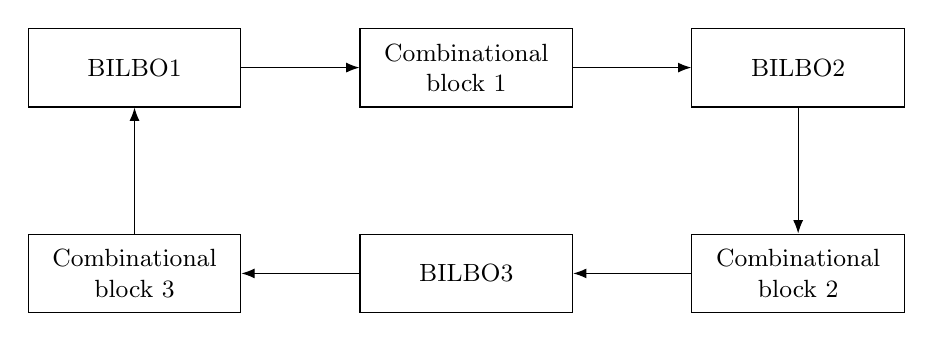
\begin{tikzpicture}[>=Latex,font=\small,b/.style={draw,align=center,minimum height=10mm,minimum width=27mm}]
\node[b] (b1) {BILBO1};
\node[b,right=15mm of b1] (c1) {Combinational\\block 1};
\node[b,right=15mm of c1] (b2) {BILBO2};
\node[b,below=16mm of b2] (c2) {Combinational\\block 2};
\node[b,left=15mm of c2] (b3) {BILBO3};
\node[b,left=15mm of b3] (c3) {Combinational\\block 3};
\draw[->](b1)--(c1);\draw[->](c1)--(b2);\draw[->](b2)--(c2);
\draw[->](c2)--(b3);\draw[->](b3)--(c3);\draw[->](c3)--(b1);
\end{tikzpicture}
\caption{The three BILBO boundaries and combinational blocks. Each BILBO has a four-bit parallel data interface.}
\end{figure}

\subsection{Explicit gate interpretation}
The photographed control labels are partly obscured by handwriting. The following interpretation states the multiplexer convention explicitly: $B_1=0$ selects ScanIn, and $B_1=1$ selects feedback. This is also visible in the clearer matching BILBO circuit supplied with the later exam. Number the flip-flops $q_1$ through $q_4$ from left to right. The feedback is
\[
F=q_2\oplus q_3\oplus q_4.
\]
Let $u$ be ScanIn when $B_1=0$ and $F$ when $B_1=1$. The depicted NOR and XOR gates give
\begin{align*}
q_1^+&=\overline{u\lor B_2}\oplus(B_1Z_1),\\
q_i^+&=\overline{q_{i-1}\lor B_2}\oplus(B_1Z_i),\qquad i=2,3,4.
\end{align*}
These equations define the rebuilt circuit without relying on a memorized BILBO mode table.
\begin{center}\small
\begin{tabular}{ccp{100mm}}
\toprule $B_1$&$B_2$&Behavior for the depicted gates\\\midrule
0&0&Inverting serial shift: $q_1^+=\overline{\mathrm{ScanIn}}$, $q_i^+=\overline{q_{i-1}}$.\\
0&1&Clear on the clock, since all four next-state values are zero.\\
1&0&Feedback with parallel response injection: an affine MISR. With all $Z_i=0$, it becomes an autonomous affine pattern source.\\
1&1&Parallel register operation, $q_i^+=Z_i$.\\
\bottomrule
\end{tabular}\end{center}

\subsection{Part (a): Source and observer}
BILBO1 must supply known patterns to block 1, and BILBO2 must compact block 1's responses. For the displayed convention, BILBO2 uses $(B_1,B_2)=(1,0)$. BILBO1 can use the same controls as a pattern source only when its parallel inputs are held at zero or equivalently isolated from response injection. Load a known initial state, accounting for the inversions in serial mode, apply the prescribed number of clocks, and compare BILBO2's final signature with the good-circuit signature for the same seed and clock count.

\textbf{Circuit limitation.} The block diagram alone does not show a mechanism that clamps BILBO1's four parallel inputs. If these inputs remain driven by combinational block 3, setting $(1,0)$ makes BILBO1 a response-fed register rather than an independent PRPG. Therefore the control pair alone does not prove the claimed independent test operation. An answer assigning $(0,0)$ to autonomous PRPG operation would also conflict with the serial-input selection and NOR gates as interpreted above. The additional input-isolation condition must be stated rather than silently assumed.

\subsection{Part (b): Polynomial and bit convention}
For $(B_1,B_2)=(1,0)$, the zero-input state update has the form
\[
q^+=Aq+\boldsymbol{1},\qquad
A=\begin{bmatrix}
0&1&1&1\\1&0&0&0\\0&1&0&0\\0&0&1&0
\end{bmatrix}
\quad\text{over }GF(2).
\]
The characteristic polynomial of its \emph{linear part} in this left-to-right state convention is
\[
\boxed{p(x)=\det(xI-A)=x^4+x^2+x+1.}
\]
Describing the same tap connection in the opposite serial/polynomial direction gives the reciprocal feedback polynomial
\[
x^4p(x^{-1})=x^4+x^3+x^2+1.
\]
Both expressions require their convention to be stated. The NOR gates add the constant vector, so the complete register update is affine rather than a purely linear LFSR. Moreover $p(1)=0$, so the linear polynomial is not primitive and a maximal 15-state linear sequence must not be claimed from this diagram.

\section{Wrapped cores, TAP control, and TAM (25 points)}
\question{Two IEEE 1500-wrapped cores connect to an IEEE 1149.1 interface. Decoder 1 produces wrapper control signals from the TAP controller and instruction register. A three-bit daisy-chain TAM carries test data. The four internal scan chains have lengths 120, 240, 240, and 120 bits. Both cores use the same operating frequency and power supply.}

\begin{figure}[ht]\centering
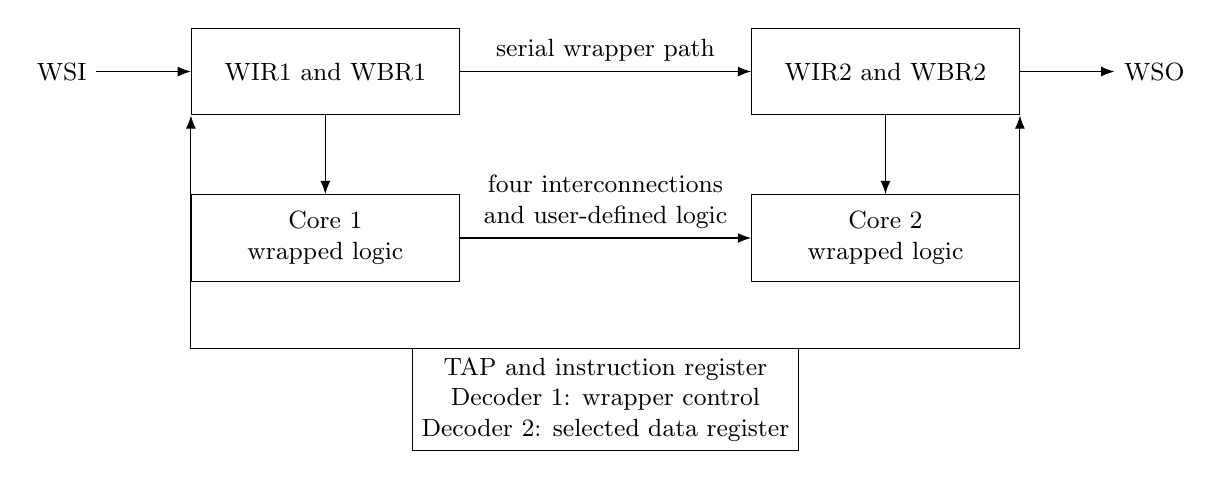
\begin{tikzpicture}[>=Latex,font=\small,b/.style={draw,align=center,minimum width=34mm,minimum height=11mm}]
\node[b] (c1) {Core 1\\wrapped logic};
\node[b,right=37mm of c1] (c2) {Core 2\\wrapped logic};
\node[b,above=10mm of c1] (w1) {WIR1 and WBR1};
\node[b,above=10mm of c2] (w2) {WIR2 and WBR2};
\node[b,below=14mm of $(c1)!.5!(c2)$] (tap) {TAP and instruction register\\Decoder 1: wrapper control\\Decoder 2: selected data register};
\draw[->](c1.east)--node[above,align=center]{four interconnections\\and user-defined logic}(c2.west);
\draw[->](w1)--(c1);\draw[->](w2)--(c2);
\draw[<-](w1.west)--++(-12mm,0)node[left]{WSI};
\draw[->](w1)--node[above]{serial wrapper path}(w2);
\draw[->](w2.east)--++(12mm,0)node[right]{WSO};
\draw[->](tap.north west)-|(w1.south west);
\draw[->](tap.north east)-|(w2.south east);
\end{tikzpicture}
\caption{Rebuilt logical organization. WIR is the wrapper instruction register and WBR is the wrapper boundary register. The parallel TAM routing is shown separately below.}
\end{figure}

\subsection{Reset without a reset input (3 points)}
\question{How can the TAP controller reset when it has no separate reset signal?}
\answer Hold TMS high for at least five rising edges of TCK. From any of the 16 TAP states, these transitions reach Test-Logic-Reset. Keep TMS high to remain there. Then apply TMS=0 on the next rising edge to enter Run-Test/Idle. The complete rebuilt transition table makes the reset path explicit.
\begin{center}\small
\begin{tabular}{lll}
\toprule Current state&TMS=0 next state&TMS=1 next state\\\midrule
Test-Logic-Reset&Run-Test/Idle&Test-Logic-Reset\\
Run-Test/Idle&Run-Test/Idle&Select-DR-Scan\\
Select-DR-Scan&Capture-DR&Select-IR-Scan\\
Capture-DR&Shift-DR&Exit1-DR\\
Shift-DR&Shift-DR&Exit1-DR\\
Exit1-DR&Pause-DR&Update-DR\\
Pause-DR&Pause-DR&Exit2-DR\\
Exit2-DR&Shift-DR&Update-DR\\
Update-DR&Run-Test/Idle&Select-DR-Scan\\
Select-IR-Scan&Capture-IR&Test-Logic-Reset\\
Capture-IR&Shift-IR&Exit1-IR\\
Shift-IR&Shift-IR&Exit1-IR\\
Exit1-IR&Pause-IR&Update-IR\\
Pause-IR&Pause-IR&Exit2-IR\\
Exit2-IR&Shift-IR&Update-IR\\
Update-IR&Run-Test/Idle&Select-DR-Scan\\
\bottomrule
\end{tabular}
\end{center}
The repository checker starts from every state and verifies that five consecutive TMS ones reach reset.

\subsection{Origins of a and p (3 points)}
\question{Do controls $a$ and $p$ come from Decoder 2 or directly from the TAP controller?}
\answer They come from the instruction-dependent decoding in Decoder 2. Control $a$ selects the wrapper/TAM data route. Multiplexer $p$ selects between that result and the bypass register. Its lower input is the bypass-register output, not the instruction-register output. The instruction register has a separate route to the final multiplexer $q$. The TAP controller instead supplies the phase of the operation, such as capture, shift, or update. The same TAP state can be used with several instructions, so state alone cannot select the instruction-dependent data-register route.

\subsection{TDO instruction/data selection q (4 points)}
\question{Explain how control $q$ is decoded.}
\answer The final multiplexer has two data inputs: the instruction-register output and the selected data-register output from $p$. It must choose the instruction register in Shift-IR and the selected data register in Shift-DR. If $q=1$ selects the instruction input, a valid decode for the observed shift phases is
\[
q=\mathbb{1}\{\text{TAP state is Shift-IR}\}.
\]
Reverse the polarity if the physical multiplexer labels use the opposite input ordering. Decode $q$ from the TAP state. A value for non-shift phases may be chosen consistently with the surrounding implementation, because no shifted bit is observed then. The expression Shift-IR OR Shift-DR would be one in both shift phases and therefore cannot select the two different sources. A separate TDO output-enable function may use those phases, but it is not the selection control $q$ drawn here.

\subsection{External testing through the serial wrapper interface (5 points)}
\question{The IEEE 1149.1 instruction 1500Test enables the wrappers. Their instructions include Bypass, InTest for core logic, and ExTest for interconnections or user-defined logic. Describe the instruction, data, and path sequence for external testing of I1--I4 using WSI--WSO.}
\answer Use the following sequence.
\begin{enumerate}
\item Reset the TAP, then use Capture-IR, Shift-IR, and Update-IR to install the 1500Test instruction. Instruction encodings are implementation-defined and are not supplied in the figure.
\item Select the wrapper instruction path. Shift the ExTest instruction for both wrappers through WSI, WIR1, WIR2, and WSO. Update the WIRs together. Keep the IEEE 1149.1 instruction at 1500Test while issuing the wrapper controls.
\item Select the wrapper data path, rather than WIR. Shift a test vector into the boundary-register scan path. Core 1's output-wrapper cells hold the values that will drive the user-defined logic. Other wrapper bits can be don't-cares where they do not affect the observed interconnections.
\item Update the output-wrapper latches to apply the vector, allow the interconnection logic to settle, and capture the response in Core 2's input-wrapper cells. The relevant functional path is Core 1 output WBR, I1--I4 and user-defined logic, Core 2 input WBR.
\item Shift out the captured boundary-register response through WSO and the selected IEEE 1149.1 data path to TDO. Compare against the expected response. Scan in the next vector while scanning out the previous response where the wrapper timing permits. Repeat update, capture, and shift until the test set is complete.
\end{enumerate}
InTest is not the correct wrapper instruction for this external test. The core's internal scan-chain contents are not the observations used to test the inter-core connections. The exact total shift length depends on the WBR configuration and bypass choices, which are not numerically specified in this question.

\subsection{External testing through the parallel TAM (5 points)}
\question{Describe the corresponding external-test procedure when data travels through the three-bit TAM.}
\answer The instruction setup is unchanged: load 1500Test through the TAP, then load and update ExTest in the WIRs. Select each wrapper's boundary-data route in the TAM test group. In the drawing the test group consists of two internal-scan outputs and a wrapper-data output. The wrapper-data route, rather than an arbitrary reassignment of all internal chains to TAM lanes, carries the external-test data.

Shift the boundary test vector through TAM In to the relevant WBR cells, update Core 1's output-wrapper latches, and capture the resulting I1--I4 response in Core 2's input-wrapper cells. Shift the captured WBR response to TAM Out, overlapping loading the next vector where supported. Wrapper capture, shift, and update remain under WCS control. The data transport changes from WSI--WSO to the selected TAM boundary-register route; the external launch and capture points remain the same. Other TAM lanes may be unused during this wrapper-only test.

\subsection{Internal-chain organization and minimum shift length (5 points)}
\question{Organize chains 1--4 through the shown TAM to minimize the internal scan-test time. Their lengths are 120, 240, 240, and 120 bits respectively.}
\answer Preserve the fixed lane connectivity shown in the diagram. Select
\[
\mathrm{TAM}_0:\ S_1(120)\longrightarrow S_3(240),\qquad
\mathrm{TAM}_1:\ S_2(240)\longrightarrow S_4(120).
\]
Both internal-scan paths have length 360. The third TAM route serves wrapper data and serial wrapper-related selections. The picture does not provide an independent third internal-scan lane or a crossbar that can freely permute the four chains among three lanes.

\begin{figure}[ht]\centering
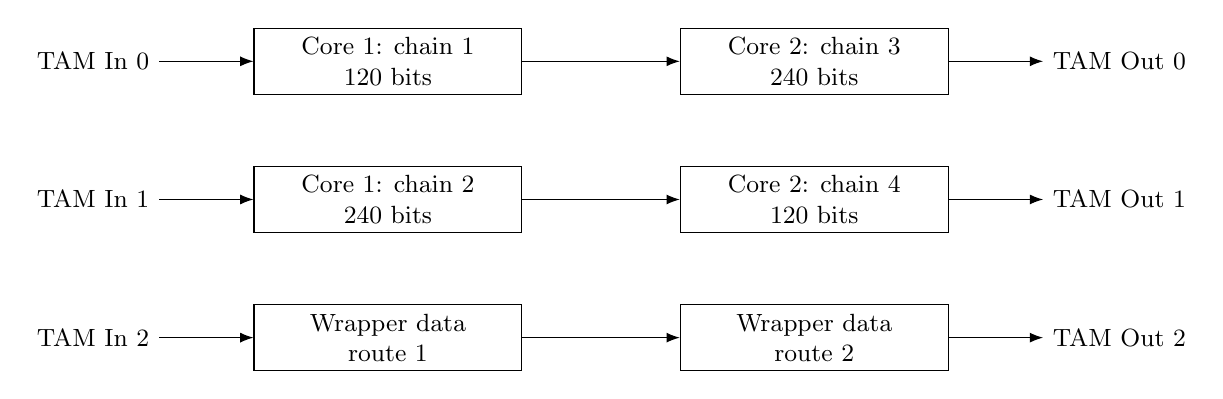
\begin{tikzpicture}[>=Latex,font=\small,b/.style={draw,align=center,minimum width=34mm,minimum height=8mm}]
\node[b] (s1) {Core 1: chain 1\\120 bits};
\node[b,right=20mm of s1] (s3) {Core 2: chain 3\\240 bits};
\node[b,below=9mm of s1] (s2) {Core 1: chain 2\\240 bits};
\node[b,right=20mm of s2] (s4) {Core 2: chain 4\\120 bits};
\node[b,below=9mm of s2] (w1) {Wrapper data\\route 1};
\node[b,right=20mm of w1] (w2) {Wrapper data\\route 2};
\foreach \a/\b/\n in {s1/s3/0,s2/s4/1,w1/w2/2}{
\draw[<-](\a.west)--++(-12mm,0)node[left]{TAM In \n};
\draw[->](\a)--(\b);
\draw[->](\b.east)--++(12mm,0)node[right]{TAM Out \n};}
\end{tikzpicture}
\caption{Shown parallel test groups. The wrapper route is not a freely assignable third internal-scan channel.}
\end{figure}

\begin{center}\small
\begin{tabular}{cll}
\toprule Control & Selection for the two 360-bit paths & Source interpretation\\\midrule
$c=0$&TAM upper lane into chain 1&$c=1$ instead selects chain 2's tail\\
$b=1$&TAM middle lane into chain 2&$b=0$ instead selects an input-WBR tail\\
$g=1$&Core 1 test output group&Fixed group: chain 1, chain 2, wrapper data\\
$j=0$&Upper group lane into chain 3&$j=1$ instead selects chain 4's tail\\
$i=1$&Middle group lane into chain 4&$i=0$ instead selects an input-WBR tail\\
$n=1$&Core 2 test output group&Export test-group data to TAM Out\\
\bottomrule
\end{tabular}
\end{center}
The 360-bit maximum is also a lower bound under these static TAM-only choices: to export Core 1 responses through its test group, chain 3 is fed either by chain 1's 120-bit route or, with the alternate local serial selection, by chain 4's 120-bit route. Either choice places at least 120 additional internal bits before its own 240 bits. The displayed selection achieves that bound without introducing a different cross-lane connection.

Let $P$ be the number of test vectors applied to the combined two-core test. With scan-out overlapped with the next scan-in, an initial fill and final drain, and one capture clock per vector,
\[
\boxed{T=360(P+1)+P\quad\text{clock periods}.}
\]
Multiply by the clock period to obtain time. This expression assumes static routing and the common test clock stated in the question. The number of patterns is not supplied, so a numerical total cannot be computed.

If a different architecture had a fully flexible three-lane crossbar, assigning $(S_1+S_4)$ to one lane and $S_2,S_3$ to the other two would give 240 bits per lane. That is an unrestricted packing lower bound. It is not an implementable answer for the multiplexers actually shown here, which do not provide the required independent lane assignment.

\section*{Verification and reconstruction limits}
The repository's standard-library checker verifies the 2020 March-test consistency choices, both transition polarities for the relevant March tests, 28 conventional two-cell single-fault March C-minus cases, and the TAP reset sequence from all 16 states. The TAM answer is based on tracing the drawn multiplexer connectivity. The BILBO answer includes an explicit gate-derived recurrence because the controls in the photographed source are partly obscured. A matching clearer circuit is used only to resolve the stated selector convention. No numerical instruction opcodes, unseen test ports, or extra scan crossbar are assumed.

\end{document}
